\documentclass[a4paper,12pt]{article} % My Personal Preference

\usepackage[table,xcdraw]{xcolor} % Prettier Tables
\usepackage[utf8]{inputenc} % Makes input utf8 (I think?)
\usepackage{amsmath} % All maths related things
\usepackage{amssymb} % Maths symbols
\usepackage{cancel} % Show cancellations in maths
\usepackage{graphicx} % Use images in your report
\usepackage{fancyhdr} % Make very nice looking header and footers for your reportthe field of study that combines biologic data with software for analysis, storage and distribution [
\usepackage{titlesec} % Change the way the default titles/heading look
\usepackage{float} % Make your pictures float/set where you want them
\usepackage[titletoc]{appendix} % Nicer appendices - acts as a section, own environment, etc.
\usepackage{siunitx} % Use SI Units in a readable manner
\usepackage{pgfplots} % Add graphs very simply
\usepackage{caption} % Options for captions
\usepackage{pdflscape} % Make landscape pages display in a PDF in landscape, instead of sideways portait
\usepackage{geometry} % ability to change the sizes of a page.  usefull for `fullbleed' pages
\usepackage{mathrsfs} % Used for Maths-based script letters (like the R for the real number set, or F for Fourier Transform)
\usepackage{listings} % format your code for pretty display
\usepackage[american]{babel} % Does something to do with formatting based on culture
\usepackage{csquotes}
\usepackage[url=true,backend=biber,style=apa]{biblatex} % better bibliographies
\DeclareLanguageMapping{american}{american-apa}
\usepackage{nameref} % Reference names and make them links (I think?)
\usepackage[backref=true,colorlinks=true]{hyperref} % Should be last package include.  Adds links that work
\usepackage[numbered,framed]{matlab-prettifier} % Pretty-print MATLAB code
\usepackage{setspace}

$if(graphics)$
\usepackage{graphicx,grffile}
\makeatletter
\def\maxwidth{\ifdim\Gin@nat@width>\linewidth\linewidth\else\Gin@nat@width\fi}
\def\maxheight{\ifdim\Gin@nat@height>\textheight\textheight\else\Gin@nat@height\fi}
\makeatother
% Scale images if necessary, so that they will not overflow the page
% margins by default, and it is still possible to overwrite the defaults
% using explicit options in \includegraphics[width, height, ...]{}
\setkeys{Gin}{width=0.9\maxwidth,height=\maxheight,keepaspectratio}
$endif$

\let\origfigure\figure
\let\endorigfigure\endfigure
\renewenvironment{figure}[1][2] {
    \expandafter\origfigure\expandafter[H]
} {
    \endorigfigure
  }

% `caption' setup
\captionsetup{justification=centering}

% Required for syntax highlighting
$highlighting-macros$

$for(bibliography)$
\addbibresource{$bibliography$}
$endfor$

\setlength{\parindent}{0pt}
\setlength{\parskip}{6pt plus 2pt minus 1pt}
\setlength{\emergencystretch}{3em}  % prevent overfull lines
\providecommand{\tightlist}{%
  \setlength{\itemsep}{0pt}\setlength{\parskip}{0pt}}

\newcommand{\dueDate}{September 7, 2018}

%Fancy Header Formatting
% This is pretty much my standard, but I move the parts around based on
% how long titles are
\pagestyle{fancy}
\fancyhf{}
\setlength{\headheight}{15pt}
\lhead{Buchan-Swanson, David}
\rhead{\dueDate}
\lfoot{Simplifying Bioinformatic Dataset Access}
\rfoot{\thepage}
\renewcommand{\footrulewidth}{0.4pt}


\begin{document}
  %--------------PREAMBLE-------------------------
  % includes the title page, gives roman numerals to all pages before the first page,
  % A titlepage template found online by David Buchan-Swanson a long time ago, and modified to fit the uses required.  If you own this, please contact me.

\begin{titlepage}

\newcommand{\HRule}{\rule{\linewidth}{0.5mm}} % Defines a new command for the horizontal lines, change thickness here

\centering % Center everything on the page

%----------------------------------------------------------------------------------------
%	HEADING SECTIONS
%----------------------------------------------------------------------------------------

\textsc{\LARGE Queensland University of Technology}\\[1cm] % Name of your university/college
\textsc{\Large Engineering Honours Thesis}\\[0.5cm] % Major heading such as course name

%----------------------------------------------------------------------------------------
%	TITLE SECTION
%----------------------------------------------------------------------------------------

\HRule \\[0.4cm]
{ \huge \bfseries Simplifying Programmatic Access to Bioinformatic Datasets}\\[0.2cm] % Title of your document
\HRule \\[.5cm]

%----------------------------------------------------------------------------------------
%	AUTHOR SECTION
%----------------------------------------------------------------------------------------

\begin{minipage}{0.45\textwidth}
\begin{flushleft} \large
\emph{Author:}\\
David \textsc{Buchan-Swanson}\\
\end{flushleft}
\end{minipage}
~
\begin{minipage}{0.45\textwidth}
\begin{flushright} \large
\emph{ID Number:}\\
n9433236\\
\end{flushright}
\end{minipage}\\[1cm]

% If you don't want a supervisor, uncomment the two lines below and remove the section above
%\Large \emph{Author:}\\
%John \textsc{Smith}\\[3cm] % Your name
\begin{minipage}{0.45\textwidth}
\begin{flushleft}\large
\emph{Supervisor:} \\
Assoc. Prof. James \textsc{Hogan}\\
[.5cm]
\emph{Unit Co-ordinator:} \\
Prof. Margot \textsc{Brereton}\\
\end{flushleft}
\end{minipage}\\[.7cm]

%----------------------------------------------------------------------------------------
%	DATE SECTION
%----------------------------------------------------------------------------------------

{\large \dueDate}\\[.5cm] % Date, change the \today to a set date if you want to be precise

%----------------------------------------------------------------------------------------
%	LOGO SECTION
%----------------------------------------------------------------------------------------


\includegraphics[width=.4\linewidth]{logo.png}\\[.8cm] % Include a department/university logo - this will require the graphicx package

%----------------------------------------------------------------------------------------

Generated using Pandoc and the \LaTeXe$\-$ typesetting system.

Note: {\color{cyan}Cyan} sections remain unchanged from the project proposal.
\vfill % Fill the rest of the page with whitespace

\end{titlepage}

  \pagenumbering{roman}
  % Changes the page style to plain - only display page number - no headers
  \pagestyle{plain}
  \doublespacing

  \section*{Executive Summary}
  \addcontentsline{toc}{section}{Abstract}
  {\color{cyan}
    Bio-informatics is an increasingly important field, and its very nature
  produces an extraordinarily large amount of data. Management and usage of
  this data becomes critical in order to achieve anything meaningful
  \parencite{lee_bioinformatics_2012}.

  A type provider is a compiler extension for F\# which allows for types to be
  programatically generated for large datasets. This makes them easier to manage
  and interact with.

  The goal for this research is to simplify access to bioinformatic data,
  starting with Genbank.  To achieve this, the aims are to explore the
  viability of a tool to simplify the processing of data, and to establish its
  usefulness in the community.

  To date, an initial implementation of an F\# type provider has been built,
  with functionality to view taxa and genomes available available on Genbank.
  There is continuing work on addtional functionality to reach usability by the
  wider community.

  Included is current progress made towards completion of the type provider,
  challenges faced in the project and an outline of future work.
  }
  \newpage

  \singlespacing
  \tableofcontents

  % then clears the page, and goes back to arabic numerals
  \newpage
  \doublespacing
  \pagestyle{fancy} % sets the page style back to nice headers
  \pagenumbering{arabic}
  \setcounter{page}{1}

  % \renewcommand{\thesection}{} % don't show a part number in the ToC
	\titleformat{\section}[hang]{\Large\bfseries}{}{0ex}{}{} % No Part Specifier in title

  $body$

  \newpage
  \printbibliography
  \addcontentsline{toc}{section}{References}

  \newpage

  \titleformat{\section}[hang]{\Large\bfseries}{}{0ex}{{\normalfont Appendix \thesection}\hspace{.5ex}\textbar\hspace{.5ex}}{}
  \pagestyle{empty}
  \begin{appendices}
    \begin{landscape}
      \section{Gantt Chart}
      \label{gantt-chart}
      \begin{figure}
        \centering
        \makebox[\textwidth][c]{
        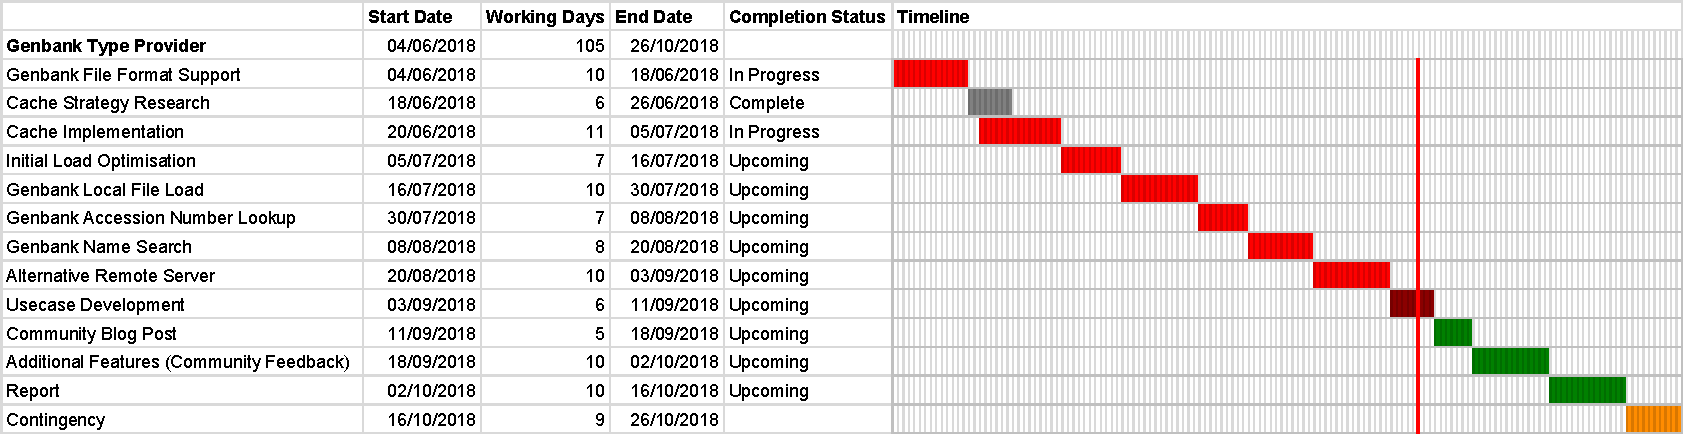
\includegraphics[width=1.5\textwidth]{src/images/ganttChart.pdf}}%
        \caption{Tasks in green are upcoming and are not due to have started
          yet, blue are in progress and within time expectations, and an orange
          contingency signifies between 5 and 10 days available.}
      \end{figure}
    \end{landscape}
  \end{appendices}

\end{document}

